\subsection*{Tilpasning af træningsniveau}
Førend træningen kan påbegyndes, tilpasses træningsniveauet den enkelte bruger. Tilpasning af træningsniveauet er inddelt i fire boundarys. Disse håndteres af en samlet controller, hvilket fremgår af \autoref{fig:DesignTilpasning}.

\begin{figure} [H]
\centering
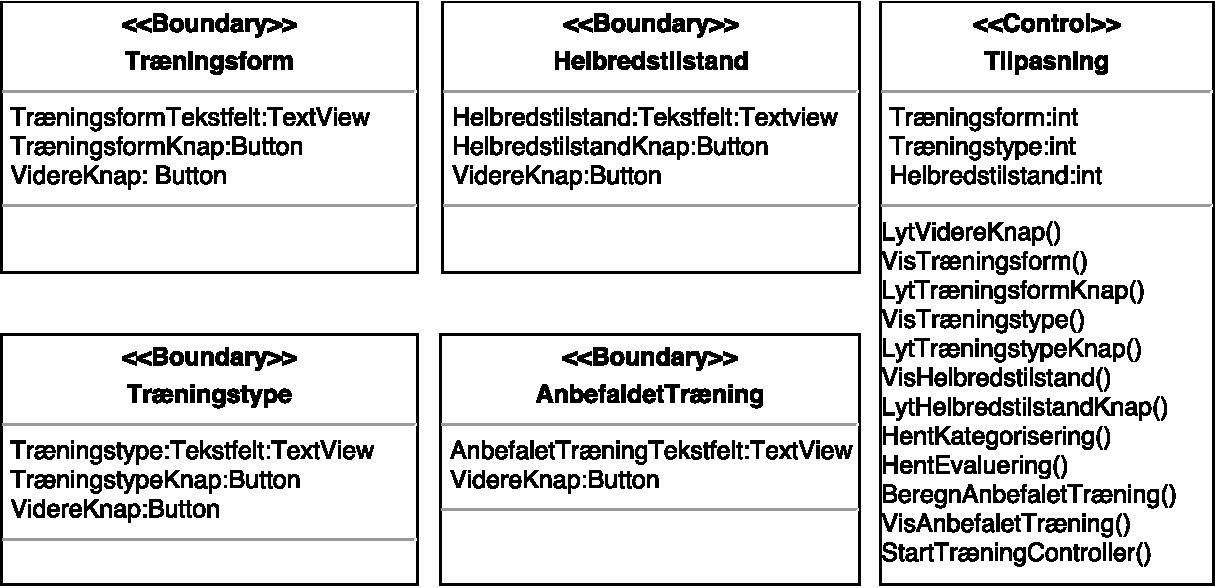
\includegraphics[width=0.9\textwidth]{figures/MVC/MVCTilpasning}
\caption{Designklasser for tilpasning af træningsniveau.Til venstre ses de fire boundarys for henholdsvis Træningsform, Træningstype, Helbredstilstand og AnbefaletTræning. Til højre fremgår den tilhørende controller.}
\label{fig:DesignTilpasning}
\end{figure}

\noindent
Der er opstillet grænseflader for tilpasning af træning, hvilket omfatter \textit{Træningsform}, \textit{Træningstype}, \textit{Helbredstilstand} og \textit{AnbefaldetTræning}. Tilpasningen af træningsniveau er delt for således at gøre app’en overskuelig samt brugervenlig. Der er til hver grænseflade opstillet tekstfelter af typen TextView og knapper af typen Button.   

Den tilhørende controller til de ovenstående boundarys lagrer den angivne træningsform, træningstype samt helbredstilstand, således disse senere kan benyttes til at beregne et passende træningsniveau. Der er dertil opstillet Vis, Lyt, Hent og Beregn-metoder til denne controller. 

Da det for brugeren skal være muligt at tilkoble kompatible enheder, forekommer endnu en controller. Denne skal håndtere kommunikation mellem systemet og kompatible måleenheder. Designklassen for kompatible måleenheder ses af \autoref{fig:kompatiblemåleenheder}.

\begin{figure} [H]
\centering
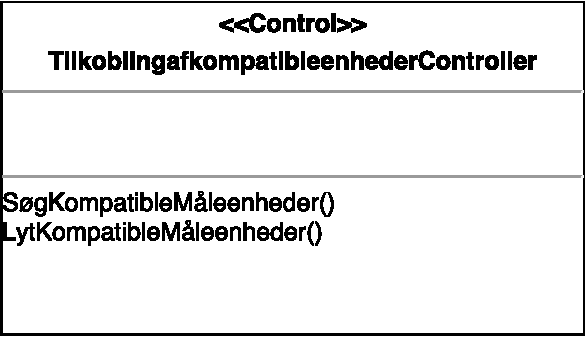
\includegraphics[width=0.5\textwidth]{figures/MVC/MVCKompMaale}
\caption{Designklasse for kompatible måleenheder. Denne er en controller.}
\label{fig:kompatiblemåleenheder}
\end{figure}

\noindent 
Denne controller tilgås ikke af brugeren, da det ønskes, at denne er en autonom funktion, der lytter efter og eventuelt tilslutter kompatible måleenheder førend en træning påbegyndes. Controlleren har en Lyt og Tilslut metode. 

I sammenspil med designklasserne er der udarbejdet et sekvensdiagram, hvilket fremgår af \autoref{fig:SEKTilpasning}. 

\begin{figure} [H]
\centering
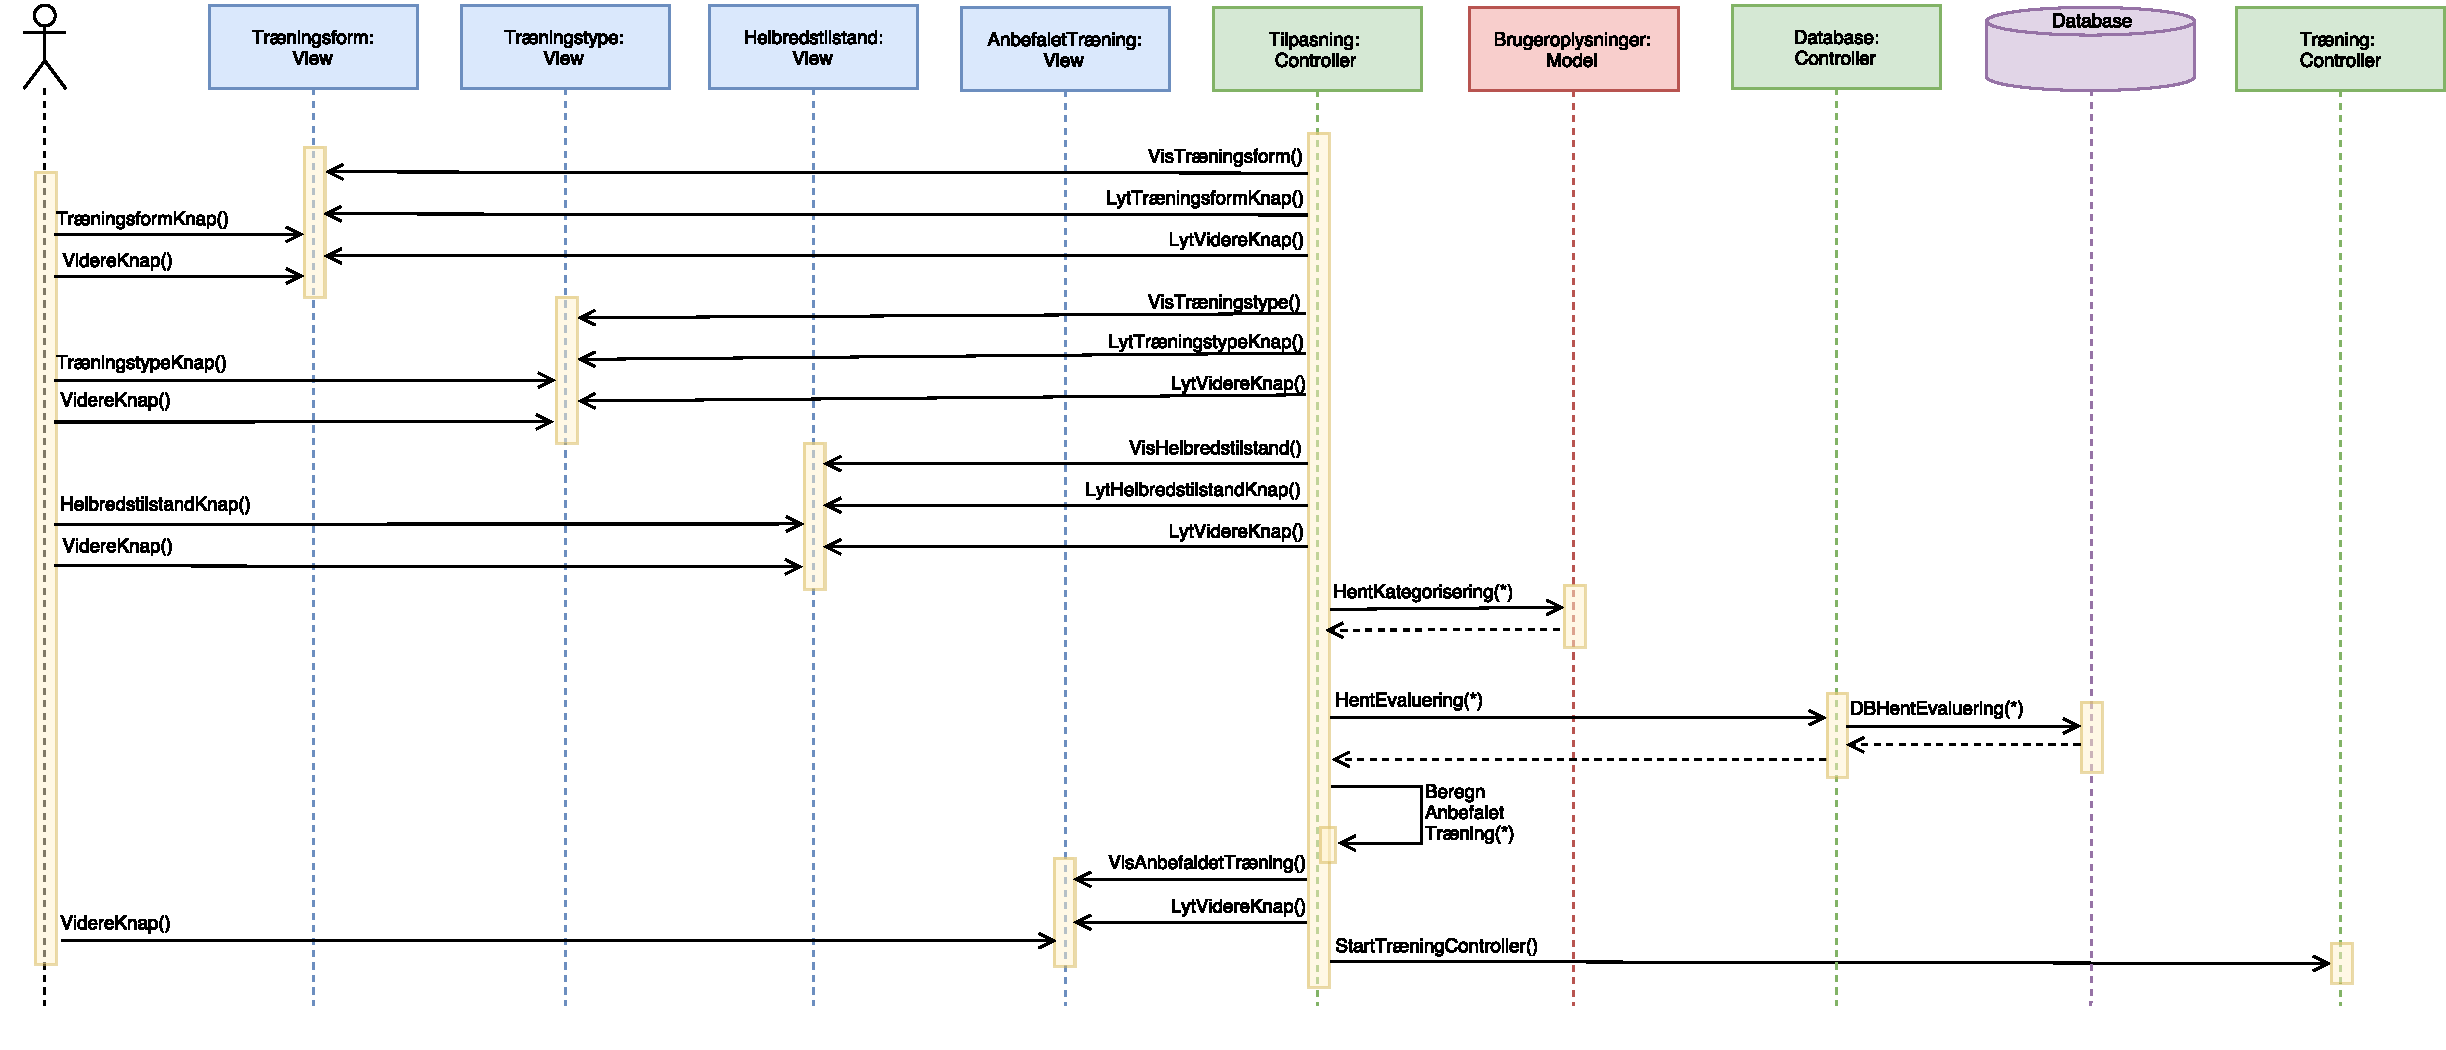
\includegraphics[width=1.5\textwidth, angle=90]{figures/Sek/SEKTilpasning}
\caption{Sekvensdiagram for tilpasning af træningsniveau.}
\label{fig:SEKTilpasning}
\end{figure}

\noindent
Den første grænseflade, som vises, er \textit{Træningsform}. Denne grænseflade indeholder et tekstfelt, der beskriver, hvad brugeren skal angive. Dertil er der opstillet en TræningsformKnap, hvor brugeren kan vælge mellem konditionstræning, styrketræning eller vejrtrækningsøvelser. Når der er angivet træningsform, trykker brugeren på VidereKnap. Hvorefter controlleren, \textit{Tilpasning}, viser grænsefladen for valg af \textit{Træningstype}. Brugeren skal her angive træningstype ud fra tre forskellige muligheder. Dette vil for eksempel ved konditionstræning være gå, løbe eller cykle. Brugeren bekræfter valget ved at trykke på VidereKnap, hvorefter controlleren viser grænsefladen for \textit{Helbredstilstand}. Helbredstilstanden angives og bekræftes ved at trykke på VidereKnap, herefter henter controlleren kategoriseringen i modellen for \textit{Brugeroplysninger} og efterfølgende evaluering i \textit{KonditionResultater}.
Controlleren lytter efter kompatible enheder fra den anden controller \textit{KompatibleEnheder}.\fxnote{OBS! Vi er stadig lidt usikre på denne del} Hvis controlleren, \textit{KompatibleEnheder}, prøver at tilslutte kompatible enheder sender denne en besked til \textit{Tilpasning} controlleren om, hvorvidt en kompatible måleenhed er tilsluttet. Hvis kompatible måleenheder tilsluttes, vil dette fremgå i grænsefladen, \textit{AnbefaletTræning}. Modsat vil det fremgå, hvis ingen kompatible måleenheder er tilsluttet. 
Efterfølgende beregner controlleren anbefalet træningsniveau og viser dette på grænsefladen for \textit{AnbefaletTræning}. Brugeren kan herefter trykke på StartKnap, hvis denne trykkes på viser controlleren grænsefladen for \textit{Træning}. 
